\section{Demonstration on the public polarization maps}
\label{sec:data}

This section does one thing: it applies the estimators of Sects.~\ref{sec:flat} and \ref{sec:profile}
to the same real maps, with the same regions, mask, bands and noise model, so that the difference
between their answers is the difference between the estimators and nothing else. It does not deliver
a polarized synchrotron index. Sect.~\ref{sec:moves} shows why not: at the statistical precision these
maps offer, analysis choices that are independent of the estimator move the index by as much as its
error or more.

\subsection{Data and model}

\paragraph{WMAP.} The nine-year low-resolution ($N_{\rm side}=16$) Stokes $Q$ and $U$ maps of the K,
Ka, Q and V bands \citep{bennett2013} with their released dense inverse noise covariance matrices,
which carry the time-correlated noise of the differential scan and de-weight the poorly constrained
transmission-imbalance modes \citep{jarosik2007,jarosik2011}. We checked them as released
(\exref{E038}): symmetric to $10^{-9}$, positive definite with no null space, a pixel noise of 2.0
to 2.2 $\muK$ in brightness temperature, and a few modes at multipoles 2 to 6 whose variance is 65 to
164 times the median. \citet{watts2023} argue from a joint reprocessing that these matrices do not
fully describe the large-scale uncertainty of the nine-year maps; we use them as released and test
the sensitivity to the modes they flag.

\paragraph{Planck.} The PR4 map at 353 GHz \citep{npipe} as the dust tracer. For it the per-pixel $Q/U$ covariance of the map file is combined over the
sub-pixels of each $N_{\rm side}=16$ pixel, and the map is the corresponding weighted average.

\paragraph{Spectra.} Each band enters through its measured bandpass. For WMAP every detector is given
unit response to a thermal spectrum and the detectors and radiometers of a band are averaged with
equal weights, which reproduces the per-radiometer effective frequencies of the WMAP team's routine
to 0.005 GHz, and the team's correction for the drift of the band centres over the mission (0.13
percent at K band) is applied. For a power law of index $-3.1$ the effective frequencies are 22.41,
32.66, 40.30 and 59.99 GHz for K to V and 28.09 GHz for the 30 GHz band. Delta bands at the nominal
WMAP frequencies would steepen a K to Ka index by about 0.06 (a calculation, not a fit). The 353 GHz
band cannot be a delta band: a modified blackbody with index 1.53 and temperature 19.6 K
\citep{planck2018xi} seen through the band is 1.12 to 1.14 times its value at 353.0 GHz, depending on
which bolometers are counted, so a delta band overstates the dust at every lower frequency by that
factor. We use the band of the polarization-sensitive bolometers.

\paragraph{Beams.} The low-resolution maps are pixel averages of maps with beams from $0.88^\circ$
(K) to $0.08^\circ$ (353 GHz). A noise-free simulation with index $-3.1$ everywhere, each band seen
through its own Gaussian beam, gives region indices biased flat by 0.005 to 0.011 for the WMAP bands
(\exref{E038}). We therefore bring every band to a common $1^\circ$ window with an invertible
operator on the $N_{\rm side}=16$ grid, $\mathsf{S}_b = 1 + \mathsf{Y}\,\mathrm{diag}(f_\ell - 1)\,
\mathsf{Y}^{+}$ with $f_\ell$ the ratio of the beam windows to multipole 47, transforming the data and
the covariance together. In the simulation the residual bias is below 0.0025, and on the real maps
the correction moves the four indices by 0.0068, 0.0025, 0.0085 and 0.0035 where the simulation
predicted 0.0070, 0.0030, 0.0088 and 0.0041 (measured with the white CMB prior, on an earlier set of
four regions and without a mask; \exref{E040}).

\begin{figure}
\centering
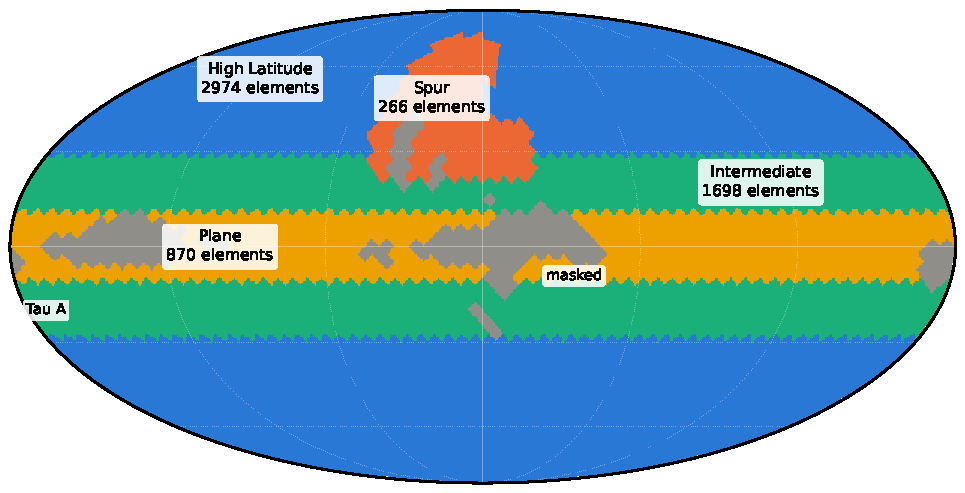
\includegraphics[width=0.85\textwidth]{figures/fig_regions.pdf}
\caption{The four regions and the processing mask (\exref{E044}), in Galactic coordinates with the Galactic
centre in the middle. An element is one Stokes parameter of one $N_{\rm side}=16$ pixel.}
\label{fig:regions}
\end{figure}

\paragraph{Regions and mask.} Four regions defined by geometry (Fig.~\ref{fig:regions}): \emph{High
Latitude}, $|b| > 30^\circ$; \emph{Intermediate}, $10^\circ \le |b| \le 30^\circ$; \emph{Plane},
$|b| < 10^\circ$; and \emph{Spur}, cut out of the first two, the northern part ($b > 20^\circ$,
$-45^\circ < l < 65^\circ$) of the pixels to which the released index map of \citet{svalheim2023}
gives its Spur value, which covers the North Polar Spur. A processing mask removes the 5 percent of
pixels with the largest polarized amplitude in the Cosmoglobe DR1 synchrotron model at 30 GHz smoothed
to $5^\circ$, which are the inner plane, the Fan region and the base of the Spur, and a disc of
$7.5^\circ$ around Tau A: \N{nkept} of \N{ntot} elements are kept, \N{nper.list} in the four regions.
\citet{svalheim2023} describe a mask of this kind for their index sampling (the strongest 5 percent of
the signal, and strong sources such as Tau A); ours follows that description and is not their file.
Masked elements are removed exactly: the kept elements enter with the inverse of their own block of
each covariance, the Schur complement of the full inverse covariance, formed after the window
matching. An earlier version of this analysis used four regions reconstructed from the released
index map without a mask; an independent referee showed that its ``High Latitude'' region held the
inner Galactic plane and that Tau A dominated the misfit of its ``Plane'' (Sect.~\ref{sec:moves}), and
those regions are not used for any statement below except where named.

\paragraph{Model.} Synchrotron as a power law with one index per region and one amplitude per
element (pixel and Stokes parameter); dust as the modified blackbody above with one amplitude per
element under a flat prior; and the CMB with one amplitude per element. The prior on the CMB
amplitudes is the $\Lambda$CDM covariance of $E$ and $B$ modes on the grid: spectra from CAMB
\citep{lewis2000} for the Planck 2018 parameters \citep{planck2018vi} with an optical depth of 0.054,
through the working window and the pixel window, for multipoles 2 to 47, the span of the harmonic
basis of the grid, plus a white floor of 0.01 $\muK$. The pixel average of a $\Lambda$CDM sky has a
further 0.11 $\muK$ per element from higher multipoles, nearly white, which this prior does not
describe (independent review, \exref{E040}); with the floor raised to that value the four indices
change by 0.0006 or less and their errors by 0.3 percent. Two other choices
are shown beside it, because the choice matters both for the index and for the pivot of
Sect.~\ref{sec:flat}: a white Gaussian prior of 0.2 $\muK$ per element, which we used first, and a
flat prior, for which the profile score is unbiased whatever the CMB is. The white prior has nearly
the right total variance (0.17 $\muK$ per element for $\Lambda$CDM) and the wrong shape: it
understates the $\Lambda$CDM $E$-mode variance by a factor of 200 at the quadrupole and overstates it
above multipole 10. With the mask, the prior on the kept elements is the kept block of that
covariance.

\paragraph{Expectations.} Expectations for every fit of this section were written down, with numbers,
before the fit was run, and the simulations of the next subsection were read before any real map
(\exref{E039}, \exref{E040}, \exref{E044}). The fits on the present regions were not the first look at
these maps: they follow a round on the earlier regions whose results we had seen, and the choice of
the $\Lambda$CDM prior over the white one was made by a rule written three minutes before the first
$\Lambda$CDM fit, after a referee had shown the white prior wrong in shape. The records mark what was
written when, and record the expectations that failed; several did, and the text says so where it
matters.

\subsection{Validation on simulations with the real covariances}

Before any fit to real data the chain was run on simulations with known indices: synchrotron
amplitudes from the Cosmoglobe DR1 polarized synchrotron map, dust amplitudes from the 353 GHz map,
a CMB drawn from the white prior, one true index per region chosen away from the centre of the allowed
range ($-3.15$, $-3.25$, $-2.85$, $-2.95$), and noise drawn from the real covariances
(\exref{E039}). Six criteria were fixed in advance. The simulations use the four regions of the earlier
version of this analysis as their geometry, and its names appear in Table~\ref{tab:e039} as labels
only; nothing tested here depends on what the regions are.

\begin{table}
\centering
\caption{Validation of the region-index estimators on simulations with the released WMAP noise
covariances (\exref{E039}): 200 noise realizations at $N_{\rm side}=8$, the first 40 with every
estimator. $z$ is the error of the profile optimum in units of the sandwich error at the truth.
The last block compares the difference between the flat-prior optima at 30 and 23 GHz with
Eq.~(\ref{eq:shift}) applied to each region alone and with the coupled form,
Eq.~(\ref{eq:coupled}), evaluated with $\J^{-1}$ in place of $\mathsf{H}^{-1}$ (the two agree here, where
$\Tm/\J$ is below 0.02).}
\label{tab:e039}
\small
\begin{tabular}{lrrrr}
\toprule
 & High Latitude & Spur & Galactic Center & Plane \\
\midrule
elements & 1124 & 212 & 50 & 150 \\
sandwich error at the truth & 0.0153 & 0.0166 & 0.0108 & 0.0146 \\
mean of $z$ & $-0.02 \pm 0.07$ & $0.00 \pm 0.07$ & $+0.07 \pm 0.07$ & $+0.01 \pm 0.07$ \\
standard deviation of $z$ & 1.04 & 0.98 & 0.94 & 1.02 \\
coverage of $\pm1\sigma$ & 0.670 & 0.715 & 0.685 & 0.695 \\
zero-mean prior minus profile, in $\sigma$ & $+0.03$ & $0.00$ & $+0.06$ & $+0.04$ \\
\midrule
flat prior at 23 GHz minus profile & $-0.0008$ & $0.0000$ & $-0.0002$ & $-0.0004$ \\
flat prior at 30 GHz minus profile & $+0.0680$ & $+0.0270$ & $+0.0074$ & $+0.0138$ \\
\quad in units of $\sigma$ & $+4.5$ & $+1.6$ & $+0.7$ & $+0.9$ \\
30 GHz minus 23 GHz, measured & $+0.0687$ & $+0.0270$ & $+0.0076$ & $+0.0142$ \\
\quad predicted, each region alone & $+0.0692$ & $+0.0156$ & $+0.0015$ & $+0.0085$ \\
\quad predicted, coupled, with $\J^{-1}$ & $+0.0723$ & $+0.0278$ & $+0.0078$ & $+0.0145$ \\
\bottomrule
\end{tabular}
\end{table}

Table~\ref{tab:e039} gives the outcome for the four regions at $N_{\rm side}=8$, where the simulated
sky is constant inside each pixel by construction. The profile optimum is unbiased to 0.07 standard
deviations, its sandwich error is right to 6 percent, the 68 percent intervals cover the truth 69
percent of the time, and the reduced $\chi^2$ at the optimum is $1.0006$ with a scatter of 0.022. A
spot check at the working resolution, $N_{\rm side}=16$, with 12 realizations gives a pooled
standardized error of mean $+0.03$ and standard deviation 0.99 and a reduced $\chi^2$ of $0.998 \pm
0.009$. The zero-mean prior lands within 0.06 standard deviations of the profile optimum. For this
band set with the white CMB prior the pivot sits at 23 GHz: a flat prior stated there is neutral, and
the same prior stated at 30 GHz moves the High Latitude index by 4.5 standard deviations. The
single-region formula predicts that move for the large region and fails for the three small ones,
which move by 1.7 to 5 times their own prediction: they are dragged by the large region through the
shared noise. The coupled form, Eq.~(\ref{eq:coupled}) with $\J^{-1}$, is within 5 percent in all four. Two of our
six criteria failed as written, one because it was worded wrongly (a lower bound of 1.0 on a ratio
that scatters around one) and one because it was written for the single-region formula. In these
regions $\Tm/\J$ is below 0.02, so the errors taken from each realization (Eq.~\ref{eq:debiased})
differ from the errors at the truth by less than a percent: with the errors taken from each of 40
realizations the standardized error has a standard deviation of 0.97 and the 68 percent coverage is
0.70, for the curvature, plug-in and debiased errors alike. The correction itself is tested in
Fig.~\ref{fig:ladder}, not here.
These simulations were first run on a numerical path that was later found to overwrite memory
(Sect.~\ref{sec:impl}); they were run again on a sound path and every number in
Table~\ref{tab:e039} and in this paragraph was reproduced to the last printed digit (\exref{E043}).

\subsection{The same maps, several answers}
\label{sec:same}

\begin{table}
\centering
\caption{The polarized synchrotron index of the WMAP nine-year K, Ka, Q and V maps (with Planck PR4
353 GHz for dust) in the four regions of \citet{svalheim2023}, at $N_{\rm side}=16$ with the dense
noise covariances, all bands brought to a common window, and the $\Lambda$CDM covariance as the prior
on the CMB (\exref{E040}). Top: the profile optimum with two errors, the debiased sandwich error,
which assumes one index per region (in parentheses for the Galactic Center, where that model does
not fit), and a block error from the scatter of the score over patches of sky, which does not (see
the text; none is quoted for the Galactic Center, where fewer than three patches carry the
information). Then the answer when the same likelihood is instead marginalized over flat
amplitude priors with the synchrotron amplitude defined at 23 or at 30 GHz, or under a zero-mean
prior with a free scale. Middle: the difference between the two flat-prior answers against
Eq.~(\ref{eq:coupled}). Bottom: goodness of fit, as $\chi^2$ per element and band, for which three
free amplitudes on five bands leave an expectation of 0.6.}
\label{tab:e040}
\small
% generated by nextgen/scripts/paperA1_make_tables.py; do not edit
\begin{tabular}{lrrrr}
\toprule
 & High Latitude & Spur & Galactic Center & Plane \\
\midrule
elements & 4388 & 928 & 182 & 646 \\
profile likelihood & $-3.082$ & $-3.080$ & $-3.081$ & $-2.964$ \\
\quad sandwich error & 0.012 & 0.016 & (0.009) & 0.013 \\
\quad block error & 0.044 & 0.038 &  & 0.100 \\
\quad effective number of patches & 5.7 & 8.8 & 2.5 & 5.1 \\
flat prior at 23 GHz & $-3.092$ & $-3.085$ & $-3.082$ & $-2.967$ \\
flat prior at 30 GHz & $-2.925$ & $-2.990$ & $-3.054$ & $-2.919$ \\
\quad minus profile, in units of the sandwich error & $+12.6$ & $+5.4$ & $+3.1$ & $+3.4$ \\
zero-mean prior, free scale & $-3.090$ & $-3.093$ & $-3.075$ & $-2.972$ \\
\midrule
flat 30 GHz minus flat 23 GHz & $+0.167$ & $+0.095$ & $+0.029$ & $+0.048$ \\
\quad Eq.~(\ref{eq:coupled}) & $+0.184$ & $+0.102$ & $+0.030$ & $+0.051$ \\
\midrule
$\chi^2$ per element and band & 0.58 & 0.59 & 1.78 & 0.77 \\
$\Tm/\J_{\rm c}$ & 0.014 & 0.005 & 0.0003 & 0.003 \\
\bottomrule
\end{tabular}

\end{table}

Table~\ref{tab:e040} is the result of this section. The numbers in each column come from the same
maps, the same regions, the same bands, the same bandpasses and the same noise covariances. They
differ only in how the amplitudes are removed.

Under flat amplitude priors the answer depends on where the amplitudes are defined. For this band set
with a $\Lambda$CDM prior on the CMB the pivot lies just above 23 GHz (23.3 to 23.4 GHz for the four
regions, to first order), and a flat prior stated at 23 GHz agrees with the profile optimum to 0.8
standard deviations. The same prior stated at 30 GHz gives
a High Latitude index of $-2.92$ instead of $-3.08$: flatter by 0.16, 12.6 standard deviations of
the sandwich error, with no change in the data or the model. The Spur moves by 0.09 and the Plane by
0.05. The difference between the two conventions is 0.91 to 0.95 of the first-order prediction,
Eq.~(\ref{eq:coupled}), in all four regions, so the identity of Sect.~\ref{sec:flat} holds on real
maps at the predicted size. The zero-mean prior with a free scale is within 0.8 standard deviations
of the profile optimum in every region.

\begin{table}
\centering
\caption{The fit of Table~\ref{tab:e040} under three priors on the CMB amplitudes: the
$\Lambda$CDM covariance, a white prior of 0.2 $\muK$ per element, and a flat prior (\exref{E040}).}
\label{tab:cmbprior}
\small
% generated by nextgen/scripts/paperA1_make_e044.py; do not edit
\begin{tabular}{lrrrr}
\toprule
 & High Latitude & Spur & Intermediate & Plane \\
\midrule
\multicolumn{5}{l}{\emph{profile likelihood, with the sandwich error}} \\
$\Lambda$CDM covariance & $-3.147 \pm 0.029$ & $-3.139 \pm 0.027$ & $-3.091 \pm 0.019$ & $-3.039 \pm 0.015$ \\
white, 0.2 $\mu$K & $-3.173 \pm 0.026$ & $-3.137 \pm 0.025$ & $-3.104 \pm 0.019$ & $-3.040 \pm 0.014$ \\
flat & $-3.041 \pm 0.062$ & $-3.122 \pm 0.060$ & $-3.017 \pm 0.044$ & $-3.038 \pm 0.035$ \\
\multicolumn{5}{l}{\emph{flat amplitude priors, synchrotron amplitude defined at 23 GHz}} \\
$\Lambda$CDM covariance & $-3.174$ & $-3.147$ & $-3.102$ & $-3.043$ \\
white, 0.2 $\mu$K & $-3.190$ & $-3.140$ & $-3.111$ & $-3.043$ \\
flat & $-1.600$$^\dagger$ & $-2.778$ & $-2.414$ & $-2.809$ \\
\multicolumn{5}{l}{\emph{flat amplitude priors, synchrotron amplitude defined at 30 GHz}} \\
$\Lambda$CDM covariance & $-2.696$ & $-2.993$ & $-2.898$ & $-2.971$ \\
white, 0.2 $\mu$K & $-2.775$ & $-3.046$ & $-2.934$ & $-2.975$ \\
flat & $-1.600$$^\dagger$ & $-2.577$ & $-1.737$ & $-2.519$ \\
\multicolumn{5}{l}{\emph{$\chi^2$ per element and band (expectation 0.60, 0.60 and 0.40)}} \\
$\Lambda$CDM covariance & 0.577 & 0.591 & 0.572 & 0.614 \\
white, 0.2 $\mu$K & 0.573 & 0.588 & 0.570 & 0.616 \\
flat & 0.385 & 0.408 & 0.372 & 0.385 \\
\bottomrule
\end{tabular}

\end{table}

\paragraph{The prior on the CMB.} The CMB has one amplitude per element like the other components,
and the index responds to what that amplitude is allowed to be (Table~\ref{tab:cmbprior}). We began
with a white prior of 0.2 $\muK$ per element and had fixed in advance that the $\Lambda$CDM covariance
would replace it if any index moved by more than one standard deviation between the two. The Plane
moved by 2.3 and the Spur by 1.0: with the white prior all four indices are steeper, by 0.012, 0.017,
0.006 and 0.031. A simulation says what to make of that (\exref{E040}): 60 skies with the synchrotron,
dust and noise of the validation above and a CMB drawn from the $\Lambda$CDM covariance, each fitted
with the three priors at $N_{\rm side}=8$. With the matched prior the estimate is unbiased and its
error is calibrated (standardized errors with mean $-0.15$ to $+0.11$ and standard deviation 0.93 to
1.14 by region). With the white prior it is unbiased on average, but the quoted error is too small by
24 to 32 percent in three of the four regions, and the 68 percent intervals cover 48 to 65 percent of
the time: the large-scale $E$ modes that a white prior does not allow move the estimate from sky to
sky, by 0.007, 0.009, 0.003 and 0.007 relative to the matched fit. With a flat prior the estimate is
unbiased and calibrated at 2.2 to 2.5 times the error. Measured against that sky-to-sky scatter and
its correlation between regions, the moves seen on the real maps at High Latitude, in the Spur and in
the Galactic Center are unremarkable (22 percent of the simulated skies lie further out), and the
move in the Plane is 4.4 standard deviations, which a $\Lambda$CDM sky does not do.
\pend{The same scatter at $N_{\rm side}=16$.} A white prior of the right total variance is therefore
not a harmless stand-in: it leaves the index unbiased and makes its error bar too small by a quarter
to a third before any misfit.

With a flat prior on the CMB the profile score is unbiased whatever the CMB is, at the price of errors
2.2 to 2.3 times larger, and the indices are $-3.03 \pm 0.03$, $-3.06 \pm 0.04$, $-3.01 \pm 0.02$ and
$-2.99 \pm 0.03$. Against the $\Lambda$CDM version, three regions are within the scatter that the
simulation gives for that difference (1.8, 0.7 and $-0.7$ of it) and the Galactic Center is 3.4 away.
The two regions whose index depends on the CMB prior by more than a $\Lambda$CDM sky allows are the
two that do not fit.

A free CMB amplitude also moves the pivot of Sect.~\ref{sec:flat}, and with it the size of the
convention effect. With a flat CMB prior and flat priors on the other amplitudes, the High Latitude
optimum of these same four WMAP bands is at $-2.51$ when the synchrotron amplitude is defined at 23
GHz and at $-1.71$ when it is defined at 30 GHz, where the profile likelihood says $-3.03 \pm 0.03$:
the pivot has moved below the K band (to 19.7 to 19.9 GHz, to first order), and both conventions
are far from it. The simulated band set of Table~\ref{tab:flat}, which includes the LFI bands, has its
pivots about 3 GHz higher in both cases and shows the same drop when the CMB is freed. The difference between
them, 0.80, is 0.92 of the first-order prediction, and the prediction is within 10 percent in every
region and for every prior in Table~\ref{tab:cmbprior}, for shifts between 0.03 and 0.8.

\paragraph{Errors that do not assume the model.} The sandwich error is the error of the estimator if
each region has one index and the noise model is right. The $\chi^2$ per element and band says that
this is close to true at High Latitude and in the Spur (0.58 and 0.59 against 0.6), 30 percent off in
the Plane and wrong by a factor of three in the Galactic Center. An error that does not lean on it
comes from the data: at the optimum the score of a region is a sum over elements, $\sum_p g_p = 0$,
and under the model the covariance of that sum is $\J + \Tm$; if the index varies inside the region
the partial sums over patches of sky scatter by more. With the 48 pixels of an $N_{\rm side}=2$ grid
as patches, $G_B = \sum_{p \in B} g_p$, the block covariance is
\begin{equation}
\widehat{\mathrm{Cov}}_{\rm block}(\hat\beta) = \J_{\rm c}^{-1}
\Big[\sum_B \frac{G_B G_B\T}{(1-h_B)^2}\Big] \J_{\rm c}^{-1},
\qquad h_B = \frac{D_B}{\sum_{B'} D_{B'}},
\label{eq:block}
\end{equation}
with $D_B = \partial G_B/\partial\beta$ the information carried by patch $B$. Without the factor
$(1-h_B)^{-2}$ this is the cluster sandwich in common use \citep{liang1986}, which is biased low when
a few clusters carry the information; with it, it is the leverage-corrected form that in linear
regression equals the delete-one-cluster jackknife variance up to a factor $G/(G-1)$ for $G$ clusters
\citep{bell2002,cameron2015}. Our estimator is not linear, so the correspondence holds to first
order, and it is exact only where neither the noise covariance nor the prior on the CMB couples
patches. Patches are treated as independent. The information is far from evenly spread: the number of
patches that would carry it if all carried the same, $(\sum_B D_B)^2/\sum_B D_B^2$ (an analogue, in
shares of the information, of the effective number of clusters of \citealt{carter2017}), is 6, 9, 3
and 5 for the four regions on the maps, out of 46, 29, 4 and 16 patches with data. A block error from
one sky is therefore itself uncertain by a third or so and should be read with the quantiles of a
$t$ distribution with few degrees of freedom \citep{bell2002,cameron2015}; for the Galactic Center we
quote none.

What a block error means needs care (independent review, \exref{E040}). It is the error of the
estimate as a measurement of the mean index of a population of exchangeable patches. For the
information-weighted mean index of the region as realized on this sky, the sandwich error is the
right one. If the index varies coherently over several patches the block error is too small (0.6 to
0.7 of the true scatter for a correlation length of two patches in a test by the reviewer). And if the
noise covariance or the prior couples patches, the patch scores are anticorrelated and the block
error is too large even when the model is true, so the ratio of block error to sandwich error under
the model has to be taken from simulations with the covariances and the prior of the fit. With
independent patches (white CMB prior, $N_{\rm side}=8$) the block error reproduces the scatter of the
estimate: the root mean square of the standardized error is 0.82, 1.20 and 1.02 at High Latitude, in
the Spur and in the Plane where 1.1 to 1.2 is expected, and the form without the leverage correction
is too small (1.39 and 1.26 in the Spur and the Plane). When the same simulations are given a true
spread of the index of 0.1 between patches, drawn anew for each realization, the sandwich error is too
small by a factor of 2.4 to 3.1 and the block error follows the scatter of the estimate about the mean
index of the region (0.59, 0.99 and 0.91). In that test the scatter of the estimate is, within 10
percent, the spread between patches divided by the square root of the effective number of patches,
added in quadrature to the sandwich error. The rule for choosing between this form and two others,
closest to one in both tests and in doubt the more conservative, was written before either test was
read; the three forms differ by 15 to 45 percent on the maps and all are in the record.

\begin{figure}
\centering
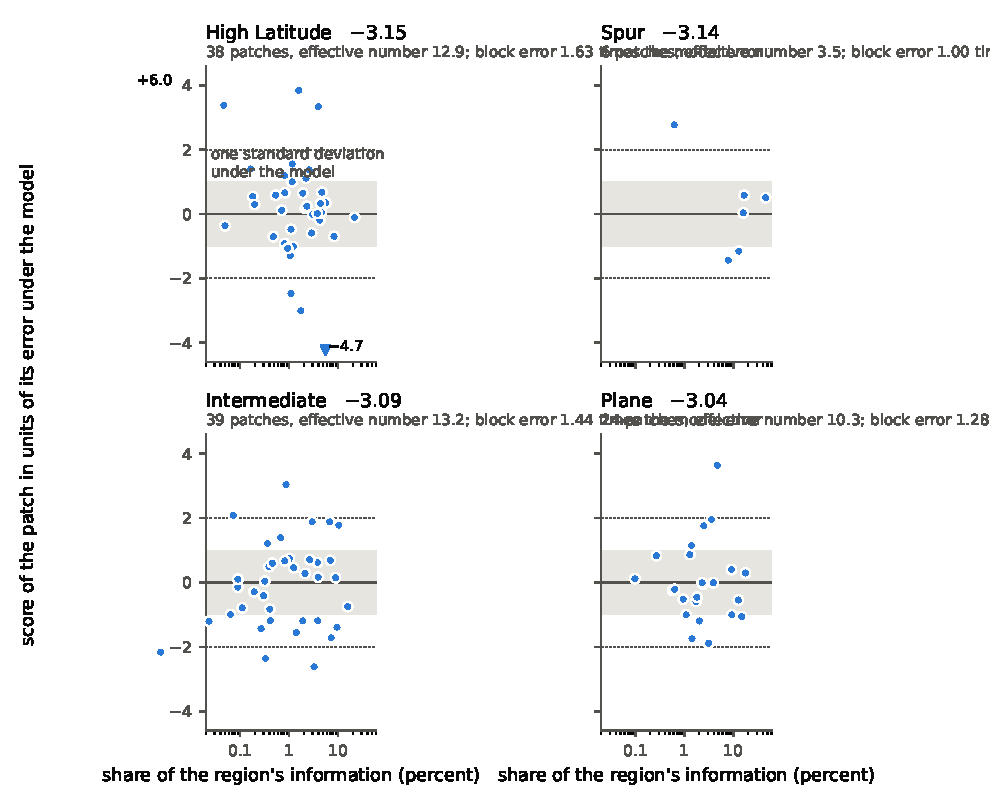
\includegraphics[width=\textwidth]{figures/fig_blocks.pdf}
\caption{What the block errors of Table~\ref{tab:e040} are made of. For each patch of sky (a pixel of the
$N_{\rm side}=2$ grid) that carries information on the index of a region: the index that the patch alone
would move to in one Newton step from the fitted index of the region, with the error it would have under
the model, against the share of the region's information that the patch carries. Patches with a one-step
error above 0.12 are not drawn, and arrows mark values outside the frame. Dark band: the sandwich error of
the region's index. Light band: its block error (none for the Galactic Center). The fitted index of the
region is given beside its name. The one-step values are first-order and for display; the block error
is computed from the scores, Eq.~(\ref{eq:block}) (\exref{E040}).}
\label{fig:blocks}
\end{figure}

On the maps the block error is 3.5, 2.3 and 7.5 times the sandwich error at High Latitude, in the
Spur and in the Plane (Table~\ref{tab:e040}, Fig.~\ref{fig:blocks}): 0.04, 0.04 and 0.10 where the
model gives 0.012, 0.016 and 0.013. Under the model, with the window-matched covariances and the $\Lambda$CDM prior of the fit, the ratio is
not one: in 60 simulations at $N_{\rm side}=8$ its median is 1.28, 1.21 and 1.32 and its largest value
2.8, 2.4 and 2.8, because that prior couples the patches (with the white prior the medians are 1.25,
1.03 and 1.07). Against that reference the maps are outside the range at High Latitude and in the
Plane, and the Spur is inside it: one simulation of 60 has a larger ratio. \pend{The same reference at
$N_{\rm side}=16$.} So the High Latitude region and the Plane are not one index each; for the Spur the
block error is an upper limit on the error and no evidence of misfit. In the simulation with a spread of 0.1 the median ratio is 3.8, 2.4 and 3.6. (That simulation has the
white prior; a spread of that size is the scale of what the High Latitude ratio asks for, and the
Plane asks for more.) What the fit of a region returns is the index of the half dozen patches that
carry its information. With the block errors the four regions do not differ from each other.

The comparison between the rows of Table~\ref{tab:e040} is differential. It does not need the model
to be right, only to be the same in every row.

\subsection{What moves the index, and why we do not quote one}
\label{sec:moves}

\begin{table}
\centering
\caption{Changes of the profile index of the WMAP K to V fit of Table~\ref{tab:e040} under analysis
choices that have nothing to do with the estimator (\exref{E040}, \exref{E042}). ``Index from $\ell \le
L$'': K band and 353 GHz keep all their modes, which with the prior on the CMB fixes the amplitudes,
and Ka, Q and V inform the
index through their harmonic coefficients at multipoles 2 to $L$ only. The window row compares two fits
with the white CMB prior, and the last row is the K, Ka fit minus the four-band fit when both are read
from multipoles up to 20. The flat-prior row repeats Table~\ref{tab:e040}. The statistical error of the
baseline is given for scale.}
\label{tab:moves}
\small
% generated by nextgen/scripts/paperA1_make_tables.py; do not edit
\begin{tabular}{lrrrr}
\toprule
 & High Latitude & Spur & Galactic Center & Plane \\
\midrule
baseline: all scales, $\Lambda$CDM CMB prior & $-3.082$ & $-3.080$ & $-3.081$ & $-2.964$ \\
statistical error (sandwich) & 0.012 & 0.016 & 0.009 & 0.013 \\
\midrule
flat amplitude prior at 30 GHz (Table~\ref{tab:e040}) & $+0.158$ & $+0.090$ & $+0.027$ & $+0.045$ \\
no window matching (white CMB prior, against its own baseline) & $+0.007$ & $+0.002$ & $+0.009$ & $+0.004$ \\
CMB prior: white, 0.2 $\mu$K & $-0.012$ & $-0.017$ & $-0.006$ & $-0.031$ \\
CMB prior: flat & $+0.055$ & $+0.025$ & $+0.073$ & $-0.024$ \\
index from $\ell \le 30$ & $-0.017$ & $-0.017$ & $-0.045$ & $-0.055$ \\
index from $\ell \le 20$ & $-0.024$ & $-0.031$ & $-0.055$ & $-0.084$ \\
index from $\ell \le 12$ & $-0.055$ & $-0.032$ & $-0.093$ & $-0.110$ \\
K and Ka only & $+0.024$ & $+0.012$ & $+0.038$ & $-0.002$ \\
dust index 1.48 in place of 1.53 & $-0.012$ & $-0.008$ & $-0.004$ & $-0.027$ \\
dust index 1.58 & $+0.011$ & $+0.007$ & $+0.004$ & $+0.025$ \\
no bandpass drift correction & $-0.001$ & $-0.001$ & $-0.001$ & $-0.001$ \\
353 GHz: all bolometers & $+0.002$ & $+0.001$ & $+0.001$ & $+0.003$ \\
delta bandpasses at the nominal frequencies & $-0.061$ & $-0.057$ & $-0.051$ & $-0.076$ \\
K and Ka only, both from $\ell \le 20$ (against the row above for $\ell \le 20$) & $+0.014$ & $+0.024$ & $+0.029$ & $+0.009$ \\
\bottomrule
\end{tabular}
% CMB prior: white, 0.2 $\mu$K: value -3.0940 -3.0965 -3.0867 -2.9950; sd 0.0121 0.0149 0.0088 0.0120; move in baseline sd -0.9 -1.0 -0.7 -2.3
% CMB prior: flat: value -3.0277 -3.0548 -3.0082 -2.9881; sd 0.0288 0.0358 0.0200 0.0300; move in baseline sd +4.4 +1.5 +8.2 -1.8
% index from $\ell \le 30$: value -3.0998 -3.0973 -3.1258 -3.0187; sd 0.0138 0.0177 0.0100 0.0147; move in baseline sd -1.4 -1.1 -5.1 -4.1
% index from $\ell \le 20$: value -3.1062 -3.1106 -3.1354 -3.0483; sd 0.0151 0.0190 0.0111 0.0156; move in baseline sd -1.9 -1.9 -6.2 -6.3
% index from $\ell \le 12$: value -3.1379 -3.1124 -3.1739 -3.0742; sd 0.0192 0.0207 0.0134 0.0168; move in baseline sd -4.4 -2.0 -10.5 -8.3
% K and Ka only: value -3.0583 -3.0683 -3.0431 -2.9664; sd 0.0159 0.0207 0.0115 0.0170; move in baseline sd +1.9 +0.7 +4.3 -0.2
% dust index 1.48 in place of 1.53: value -3.0949 -3.0879 -3.0850 -2.9916; sd 0.0126 0.0165 0.0089 0.0135; move in baseline sd -1.0 -0.5 -0.5 -2.1
% dust index 1.58: value -3.0713 -3.0726 -3.0769 -2.9395; sd 0.0124 0.0164 0.0088 0.0131; move in baseline sd +0.9 +0.4 +0.4 +1.9
% no bandpass drift correction: value -3.0837 -3.0810 -3.0819 -2.9655; sd 0.0125 0.0165 0.0089 0.0133; move in baseline sd -0.1 -0.1 -0.1 -0.1
% 353 GHz: all bolometers: value -3.0809 -3.0789 -3.0802 -2.9607; sd 0.0125 0.0165 0.0088 0.0133; move in baseline sd +0.1 +0.1 +0.1 +0.3
% delta bandpasses at the nominal frequencies: value -3.1438 -3.1371 -3.1319 -3.0398; sd 0.0129 0.0170 0.0091 0.0138; move in baseline sd -4.9 -3.5 -5.8 -5.7
% K, Ka against four bands at l <= 20, in units of sqrt(sd_sub^2 - sd_full^2): +1.3 +1.8 +3.4 +0.8
% start at -2.7: change -0.00000 -0.00000 -0.00000 +0.00000

\end{table}

% generated by nextgen/scripts/paperA1_make_tables.py (prose template there; numbers from the result files)
Table~\ref{tab:moves} lists what else moves the answer in the central configuration. The rows are
changes of the index; the statistical error of the baseline is given for scale.

\paragraph{Angular scale.} To ask at which scales two bands disagree we first marginalized the modes of
one map at multipoles 2 to $L$ and refitted, with the same cut in the K, Ka fit as a control fixed in
advance, where nothing should move. The control failed: the K, Ka index moved toward flat in every
region, by $+0.08$, $+0.16$, $+0.11$ and $+0.37$ at $L = 20$ (white CMB prior; \exref{E042}). Read from
the other side, with the pixel scale excluded and the index informed by multipoles up to 30, 20 or 12
only, the four-band index steepens (Table~\ref{tab:moves}): by 0.017 to 0.055 at High
Latitude, 0.017 to 0.032 in the Spur, 0.045 to 0.093 in the Galactic Center
and 0.055 to 0.110 in the Plane. The estimator is sound: on simulations with known indices it
is unbiased and calibrated (standardized errors of standard deviation 0.95 to 1.03 over 100
realizations at $N_{\rm side}=8$), an independent review re-derived it and confirmed it on its own
simulations, and the difference between the large-scale and the all-scale estimate of one simulated
sky has zero mean and a spread of 0.9 to 1.1 times $(\sigma_{\rm low}^2 - \sigma_{\rm all}^2)^{1/2}$
(\exref{E039}). On the maps the differences at $L = 20$ are 2.8, 3.3, 8.2 and 10.4 times that number. The
shifts are the same within 0.025 with the white CMB prior. So the dependence on scale is a property of
these maps under this model, in every region, and not of the estimator or of the CMB prior. An index
read from the three cuts is not stable either: the largest difference between two cuts is
2.8, 2.0, 5.4 and 6.7 times the standard deviation expected for nested fits.

We do not know the cause. One candidate is instrumental: the maps are pixel averages of skies that are
not band-limited, structure below the pixel scale folds into it through each band's own beam, K band
has the widest, and the window operator works to multipole 47 with Gaussian beams. Against it, the one
simulation we have of sub-pixel structure leaves a residual of 0.002, though that sky had no compact
sources. The other candidate is the sky: compact structure in the plane may be flatter than the diffuse
emission, and an index that varies from patch to patch (previous subsection) makes an index from
large scales and an index from all scales weight the sky differently. \citet{fuskeland2014}, with maps
smoothed to a common $1^\circ$ beam before any pixel averaging, find $-2.98 \pm 0.01$ in the plane,
close to our all-scale K, Ka value there ($-2.97$) and not to the large-scale one ($-3.04$ at
$L = 20$); that favours the sky. The rows of Table~\ref{tab:moves} are sizes of an effect and not
corrections.

\paragraph{Band subset.} K and Ka alone give indices that differ from the four bands together by
$+0.024$, $+0.012$, $+0.038$ and $-0.002$. The two fits share K and Ka, so the standard deviation of their difference
under the model is $(\sigma_{\rm sub}^2 - \sigma_{\rm full}^2)^{1/2}$, and the differences are
$+2.5$, $+0.9$, $+5.2$ and $-0.2$ of it; with both fits read from multipoles up to 20 they are
$+1.3$, $+1.8$, $+3.4$ and $+0.8$. With the white CMB prior the shifts were larger and all of one
sign ($+0.032$, $+0.023$, $+0.041$ and $+0.015$). What remains with the $\Lambda$CDM prior is a flatter K
to Ka index at High Latitude and in the Galactic Center, where the model does not fit in any case. A
spectrum that steepens with frequency would do this, and so would a dust model that predicts too much
polarized dust at 41 and 61 GHz from 353 GHz.

\paragraph{Dust.} The dust spectrum is fixed. Changing its index by 0.05 either way moves the
synchrotron index by 0.012, 0.008, 0.004 and 0.026, linearly ($\partial\beta_{\rm s}/\partial\beta_{\rm d} =
0.24$, $0.15$, $0.08$ and $0.52$): one statistical standard deviation at High Latitude
and two in the Plane, more than we had written down in advance for three of the four regions. With the
uncertainty of the Planck value, 0.02,
it is 0.005 at High Latitude and 0.010 in the Plane.

\paragraph{Bandpasses.} Leaving out the correction for the drift of the WMAP band centres changes the
index by 0.001, and taking the 353 GHz band of all bolometers in place of the
polarization-sensitive ones by 0.001 to 0.003. Replacing the measured bandpasses by delta functions at
the nominal WMAP frequencies steepens it by 0.051 to 0.076, 3.5 to 5.8 statistical standard
deviations: the effective frequency of K band for a spectrum this steep is 22.4 GHz, not 22.8.

\paragraph{Poorly measured modes.} The released K-band covariance has 20 eigenmodes with more than
ten times the median variance. Projecting all of them out moves the K, Ka index by 0.002 to 0.015
(white CMB prior). This tests the modes the matrix knows about, not the claim that it understates
them.

Taken together: for these maps and regions the profile index of the simple model is $-3.08$ at High
Latitude, in the Spur and in the Galactic Center and $-2.96$ in the Plane. Its error is 0.01 to 0.02
if each region has one index and 0.04 to 0.10 from the scatter between patches. It moves by
0.01 to 0.07 with the prior on the CMB, by 0.02 to 0.11 with the angular scales that
inform it, by up to 0.04 with the band subset, by 0.004 to 0.026 for 0.05 in the dust index, and by
0.05 to 0.08 if the bands are taken at their nominal frequencies. A number with an error bar that
means what it says needs a model in which a region is more than one index and the scale dependence
understood. That is a separate piece of work, and we do not quote an index here.


